\section{A Seiva da Árvore \ldots}\label{sec:seiva} %==========================

\begin{margintable}\vspace{.8in}\footnotesize
  \begin{tabularx}{\marginparwidth}{|X}
    Seção~\ref{sec:seiva}. A seiva da árvore\\
    Seção~\ref{sec:seiva}. A seiva da árvore\\
    Seção~\ref{sec:seiva}. A seiva da árvore\\
  \end{tabularx}
\end{margintable}

Lembro-me da primeira vez que vi o nome \LaTeX{} \ldots

Foi em uma chamada de um minicurso de alguma "semana de matemática" da 
universidade que fiz graduação.
O título era algo assim: "Introdução ao \LaTeX".

Eu estava a um semestre de concluir a graduação e pensei: 
\textit{
  "Rapaz \ldots acho que eles erraram esse minicurso. 
  Pra quê estudar látex em Matemática? 
  Isso está mais para Geografia."
}

\begin{marginfigure}
  \centering
  \href
  {
    https://www.globo.com/GloboRural/0,6993,EEC1703411-1935,00.html
  }
  {
    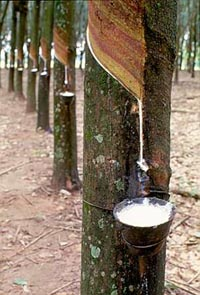
\includegraphics[width = 0.75\linewidth]{seringueira.jpg}
  }
  \caption{Isso é látex, não \LaTeX}
\end{marginfigure}

Sim! 
Eu pensei que estavam falando daquela substância espessa e branca que sai de 
algumas plantas (seringueira, por exemplo)!

Então, vamos deixar as coisas claras: não estamos falando de látex, mas de \LaTeX.

\begin{atencao}{Como pronunciar corretamente?}{\exclamacao}
  Aliás, como se pronuncia a palavra \LaTeX?\\
  Existem, pelo menos, duas maneiras de pronunciarmos, corretamente, essa palavra:
  "\textit{LeiTéc}" ou "\textit{LaTéc}", ou seja, o som de \TeX{} ("Téc") é o 
  mesmo que na palavra "\textit{tec}nologia". 
  Particularmente, adoto a segunda opção.
  Evite, por amor a Deus, falar "\textit{Látecks}".
\end{atencao}

Falando nisso, essa palavra \TeX{} não está destacada de forma aleatória! 
Ela foi idealizada como sendo a junção de três letras gregas: $\tau\epsilon\chi$.
\sidenote{%
  \footnotesize $\tau$ (tau), $\epsilon$ (épsilon) e $\chi$ (chi)
}
Esse núcleo grego gera palavras como \textit{arte} ($\small\tau\epsilon\chi\nu\eta$) 
ou mesmo \textit{tecnologia} ($\small\tau\epsilon\chi\nu o \lambda o \gamma\iota\alpha$).
Daí vem o espírito da palavra \TeX: unir uma arte (a tipografia) com a tecnologia 
(programação) para produzir documentos com uma beleza realmente ímpar.

Na realidade, para falarmos com propriedade sobre \LaTeX, precisamos tangenciar 
o \TeX.

\subsection{Diferenciando os nomes} %------------------------------------------

Tudo começou quando \href{https://pt.wikipedia.org/wiki/Donald_Knuth}{Donald Ervin Knuth} 
queria qualidade nos elementos tipográficos de seus livros, principalmente na 
escrita matemática. 
Ele então criou, em meados da década dos anos 70, um sofisticado programa para a 
composição tipográfica de textos científicos e uma alternativa quase necessária 
para edição de textos com conteúdo matemático. 
Nasceu o \TeX. 
Em suas próprias palavras:

\begin{cita}
  \TeX{} é destinado para a criação de belos livros - e, especialmente, para os 
  livros que contêm grande quantidade de matemática.
\end{cita}

Todavia, ao que parece, essa linguagem de programação não era tão acessível 
\sout{a meros mortais como nós}, por conter diversos parâmetros relativos ao 
formato final do texto \ldots
Bom, vamos falar a verdade: dava muito trabalho para digitar o que você queria 
simplificar.
Isso porque o \TeX{} era formado por objetos denominados "primitivos" e toda 
estruturação do texto deveria ser feita por meio deles.
O próprio Knuth criou um conjunto de macros\nota{
  Uma \textit{macro} (abreviação para macroinstrução), em ciência da computação, 
  é uma regra ou padrão que especifica como uma certa “sequência de entrada” 
  deve ser mapeada para uma substituição de “sequência de saída” de acordo com 
  um procedimento definido.
}, ou seja, um mapeamento de sequências de comandos primitivos, frequentemente 
utilizados, para simplificar a escrita de comandos \TeX{} em seus livros.
A esse conjunto de macros ele deu o nome de \textit{Plain}~\TeX.

Obviamente, o \textit{Plain}~\TeX{} é um conjunto de macros bem simples e que 
poderia ser expandido.
E foi isso que aconteceu.

\subsection{O surgimento do \LaTeX} %------------------------------------------

\href{https://pt.wikipedia.org/wiki/Leslie_Lamport}{Leslie B. Lamport}, facilitou 
nossa vida! 
Por volta dos anos 80, ele criou um conjunto de macros para o \TeX, muito bem 
estruturado, e com ideias interessantes (classes e pacotes, por exemplo) que 
somaram substanciamente à causa do \TeX{}, formando assim o \LaTeX.
Inclusive, o "La", de \LaTeX{}; vem do "La", de \textit{\textbf{La}mport}.
\sidenote{
  $\text{\LaTeX} = \text{\textbf{La}mport} + \text{\TeX}$
}

Logo, nunca se esqueça disso:

\begin{center}
  \Ovalbox{
    \large  \textsf{O} \LaTeX\ \textsf{veio para facilitar sua vida}!
  }
\end{center}

\begin{figure}[!ht]
  \centering
  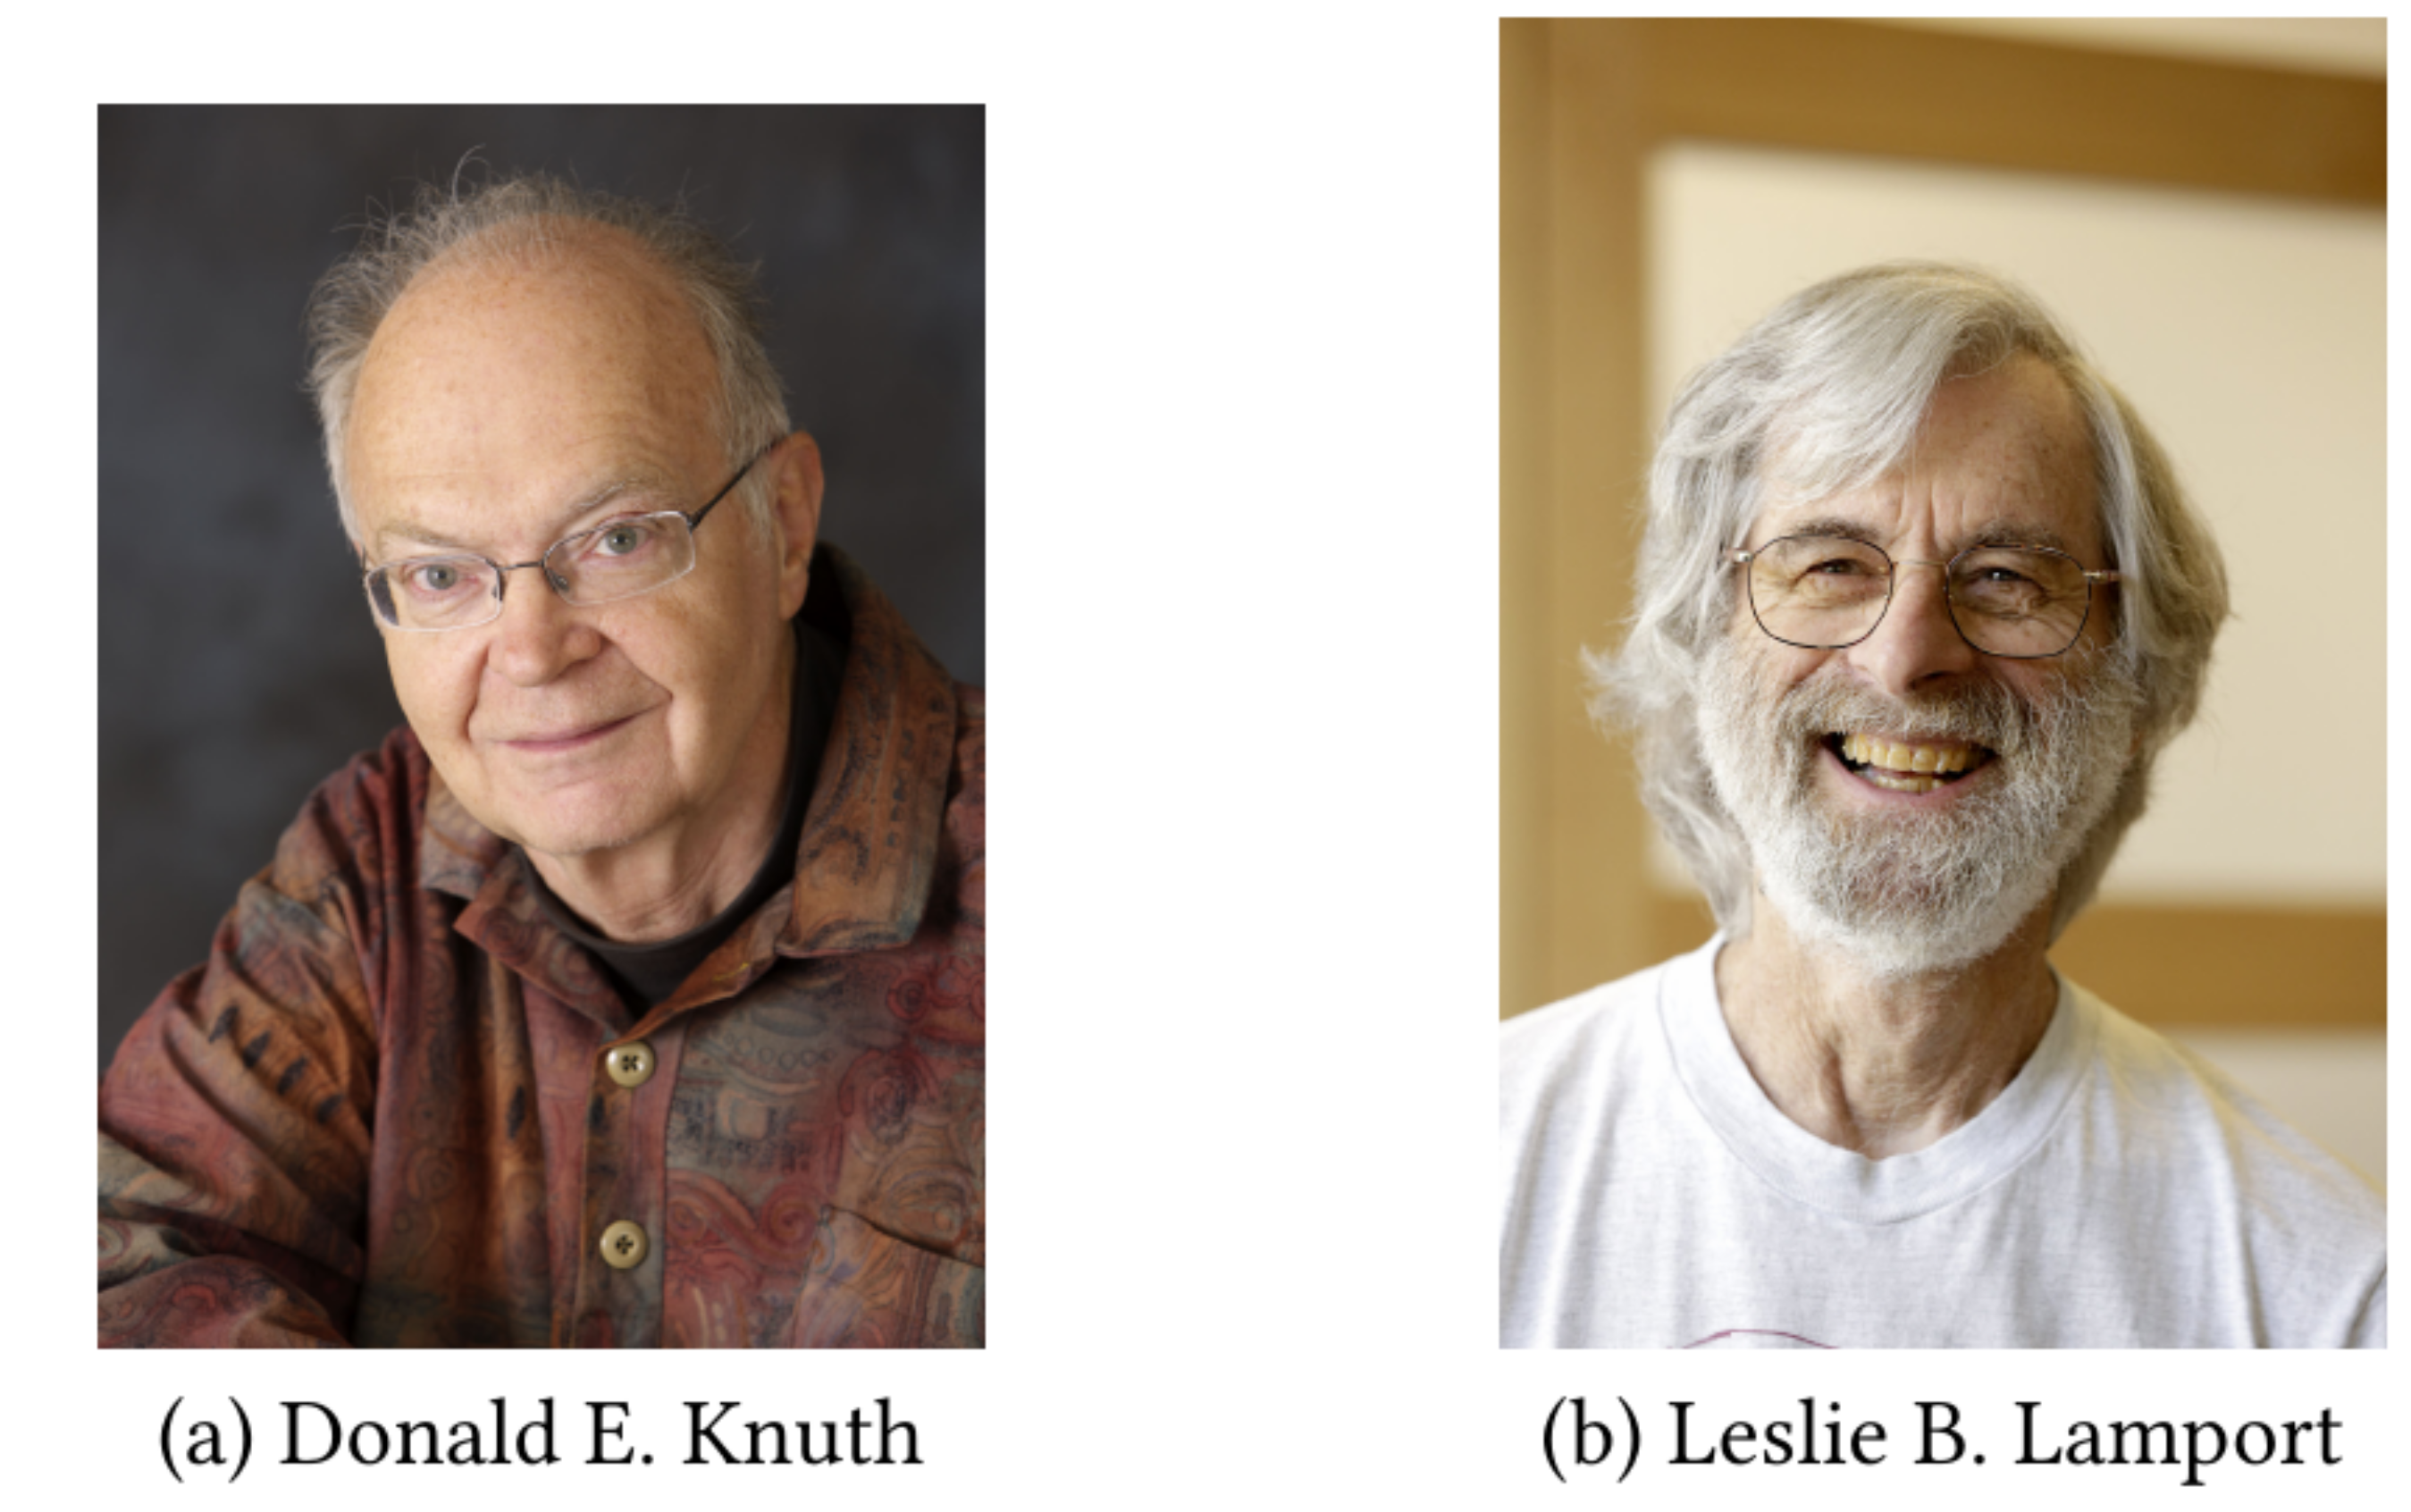
\includegraphics[width = 0.8\linewidth]{lamport-knuth}
  \caption{Os culpados!}
\end{figure}

\subsection{Mais e mais nomes: compiladores, interpretadores e formatos} %-----

Bom \ldots já sabemos que  \TeX{} e \LaTeX{} são coisas diferentes, entretanto,
interrelacionadas: o segundo é a forma mais utilizada, atualmente, para 
interagir com o primeiro.

Nesse ponto, seria interessante diferenciarmos \textit{engines} (motores/interpretadotes) 
de \textit{formats} (formatos).

O \TeX{} é um interpretador (\textit{engine}); o \LaTeX, um formato (\textit{format}).

\nota{
  Um outro formato que vimos é o \textit{Plain}~\TeX; e, atualmente, um formato 
  que se destaca é o \href{https://en.wikipedia.org/wiki/ConTeXt}{\textcolor{azulUFRB}{\hologo{ConTeXt}}}.
}

Os \textit{interpretadores} são os arquivos binários executáveis (ou seja, o 
programa em si); já os \textit{formatos} são macros (comandos ou instruções), 
baseadas em \TeX, que usamos para escrever nossos documentos (a grosso modo, são
linguagens ou atalhos para sequências de comandos ou estruturas em \TeX).

Não
\begin{marginfigure}
  \centering
  \href
  {
    https://www.lua.org/portugues.html
  }
  {
    
\includegraphics[width = 0.6\linewidth]{logo_lua.png}
  }
  \caption{Poderosa linguagem de programação (clique na imagem para saber mais)}
  \label{fig:lua}
\end{marginfigure}
é difícil perceber que o interpretador \TeX{} é bem antigo e que outros tenham
surgido ao longo desses anos.
De fato, à época do \TeX, nem existia ainda arquivos com extensão  \texttt{.pdf} 
-- a saída dos documentos era em DVI.
Quando surgiu o PDF, um interpretador ficou bem conhecido: \hologo{pdfTeX} -- cuja 
saída poderia ser em DVI que poderia ser convertida em PDF. 
O \hologo{pdfTeX} talvez seja o mais usado dentre os interpretadores que vamos 
falar, pois já vem selecionado, por padrão, em muitos editores dedicados ao 
\LaTeX \mn{%
  falaremos sobre editores para \LaTeX{} mais abaixo.}; 
as pessoas, simplesmente, não mudam a configuração padrão se realmente não 
for necessário.
Aliás, nosso sistema relaciona o \LaTeX{} com o \hologo{pdfTeX} usando um "atalho", 
denominado \hologo{pdfLaTeX}.

Portanto, o \hologo{pdfLaTeX} (que geralmente é o nome que aparecerá em nossos 
editores) é o \textit{interpretador} pdf\TeX\ com o \textit{formato} \LaTeX. 

Atualmente, dois interpretadores que se destacam são \hologo{XeTeX} e \hologo{LuaTeX}.
Além de serem mais rápidos, trazem implementações notáveis como seleção de fontes 
do próprio sistema (o \hologo{pdfTeX} não faz isso) ou interação com a linguagem 
de programação (brasileira) Lua (veja a Figura~\ref{fig:lua}). 
\nota{
  De acordo com Joseph Wright, usamos a palavra "compilação" herdada da computação,
  mas, uma palavra mais adequada seria "composição tipográfica" \cite{learnlatex}.
}
A saída de cada um deles é o PDF, diretamente.

Em nossos sistemas, ao usarmos \hologo{XeTeX} com \LaTeX{} usamos o atalho 
\hologo{XeLaTeX}.
Da mesma forma, \hologo{LuaTeX} com \LaTeX{} é simplificado por \hologo{LuaLaTeX}.

Obviamente, nesse minicurso, estamos interessados apenas no formato \LaTeX.
Também, por mera preferência, usaremos como interpretador o \hologo{LuaTeX}.
Portanto, "compilaremos" \, nossos arquivos com \texttt{lualatex}.

Obtamos por usar \lualatex, pois é o sucessor natural do \texttt{pdflatex}. 
\sidenote{
  \footnotesize
  Confira essa informação no site \href{http://www.luatex.org/}{\textbf{http://www.luatex.org/}}
}

\begin{atencao}{Mudanças à vista \ldots}{\exclamacao}
  Isso pode mudar algumas coisas para quem é acostumado a usar \texttt{pdflatex}, 
  mas explicaremos as diferenças ao longo desse minicurso.  
\end{atencao}

Geralmente chamamos esses "atalhos" de \textbf{compiladores}
\mn{
  Para mais detalhes, veja \textcite{lualatex-doc}.
}.

Veja a Tabela~\ref{tab:compiladores} para comparação entre \textit{compiladores}, 
\textit{engine} e \textit{format}.

\begin{table}[!htbp]
  \centering
  \begin{tabular}{llc}
    \toprule
      \textbf{Compilador} & \textbf{Interpretador} & \textbf{Formato} \\
    \midrule
      \texttt{tex}           & \hologo{TeX}    & \hologo{plainTeX}       \\
      \texttt{pdftex}        & \hologo{pdfTeX} & \hologo{plainTeX}       \\
      \texttt{xetex}         & \hologo{XeTeX}  & \hologo{plainTeX}       \\
      \texttt{latex}         & \hologo{pdfTeX} & \LaTeX                  \\
      \texttt{pdflatex}      & \hologo{pdfTeX} & \LaTeX                  \\
      \texttt{xelatex}       & \hologo{XeTeX}  & \LaTeX                  \\
      \texttt{lualatex}      & \hologo{LuaTeX} & \LaTeX                  \\
      \texttt{texexec}       & \hologo{pdfTeX} & \hologo{ConTeXt}        \\
      \texttt{texexec --xtx} & \hologo{XeTeX}  & \hologo{ConTeXt}        \\
      \texttt{context}       & \hologo{LuaTeX} & \hologo{ConTeXt}        \\
    \bottomrule
  \end{tabular}
  \caption{Dando "nome aos bois"}
  \label{tab:compiladores}
\end{table}

Como 
\begin{marginfigure}
  \centering
  \href
  {
    http://www.luatex.org/
  }
  {
    
\includegraphics[width = 0.9 \linewidth]{logo_luatex.png}
  }
  \caption{
    Saiba mais sobre o \hologo{LuaTeX} acessando o link: 
    \href{http://www.luatex.org}{http://www.luatex.org}
  }
  \label{fig:lua}
\end{marginfigure}
esse texto é uma \sout{tentativa de} introdução ao \LaTeX, não chegaremos 
nem perto do que gostaríamos de expor sobre essa simbiose entre uma linguagem de 
\textit{programação} (Lua) integrada harmoniosamente com uma linguagem de 
\textit{marcação} (\LaTeX).
Basicamente, o código do \TeX{} foi reescrito em Lua (uma linguagem de programação
com muita relevância internacional, desenvolvida por brasileiros, na PUC-RJ), 
formando assim o \hologo{LuaTeX}.
Houve, intencionalmente, a projeção para que esse \textit{interpretador} fosse 
compatível com versões anteriores do \hologo{pdfTeX}, tornando o \hologo{LuaTeX} 
seu substituto natural, visto que é mais rápido e moderno.

Para encerramos essa subseção, é importante destacar a estabilidade do \LaTeX.
Basicamente temos duas versões: uma antes de 1993, a saber \LaTeX~2.09; e,
a de 1994 até HOJE, a saber \hologo{LaTeX2e}.
Isso é interessante, pois os códigos são praticamente preservados ao longo do 
tempo: você poderia rodar um código em \LaTeX\ de 20 anos atrás sem muitos 
problemas.

Todavia, quando falamos em \LaTeX{}, hoje, estamos nos referindo às 
funcionalidades trazidas na versão \hologo{LaTeX2e}.

\begin{marginfigure}
  \centering
  
\includegraphics[width = \linewidth]{logo_latex}
  \caption{
    Saiba mais sobre esse fantástico projeto no link:
    \href{https://www.latex-project.org}{https://www.latex-project.org}
  }
  \label{fig:latexiii}
\end{marginfigure}

As atualizações são constantes, mas sem muitas mudanças estruturais.
Todavia, está em desenvolvimento uma terceira versão do \LaTeX, a saber, 
\hologo{LaTeX3} (veja a Figura~\ref{fig:latexiii}).

%------------------------------------------------------------------------------
\subsection{Como colocar o \hologo{LaTeX} em meu computador: as Distribuições}
%------------------------------------------------------------------------------ 

Para instalar localmente (em nosso computador) os \textit{interpretadotes}, 
precisamos das \textbf{distribuições}.

As principais são:

\begin{table}[!htbp]
  \centering
  \begin{tabular}{lll}
    \toprule
      \textbf{Distribuições} & \textbf{Sistema} & \textbf{\textit{Download}/Instalação}\\
    \midrule
      \hologo{MiKTeX}   & Windows ou GNU/Linux ou Mac OS & \href{https://miktex.org/download}{https://miktex.org/download} \\ 
      \TeX{} Live       & GNU/Linux ou Windows  & \href{https://www.tug.org/texlive/acquire-netinstall.html}{https://www.tug.org/texlive/acquire-netinstall.html}\\
      Mac\TeX           & Mac OS                & \href{https://www.tug.org/mactex/}{https://www.tug.org/mactex/}  \\
    \bottomrule
  \end{tabular}
\end{table}

A distribuição Mac\TeX{} contém todo o \TeX{} Live e adições específicas para 
Mac~OS.
\nota{
  Para GNU/Linux existem outras opções de instalação que economizam espaço.
  Tudo dependerá da necessidade de cada um:\\
  \texttt{texlive-latex-base}\\
  \texttt{texlive-latex-recommended}\\
  \texttt{texlive-pictures}\\
  \texttt{texlive-fonts-recommended}\\
  \texttt{texlive}\\
  \texttt{texlive-plain-generic}\\
  \texttt{texlive-latex-extra}\\
  Para mais informações veja essa discussão no \href{https://tex.stackexchange.com/questions/245982/differences-between-texlive-packages-in-linux}{\textcolor{azulUFRB}{TeX SE}}
}

O \TeX{} Live completo precisa de, aproximadamente, 5GB de espaço em disco.
Ele instala TODOS os pacotes disponíveis para \hologo{LaTeX}.
Como hoje em dia a capacidade de disco é relativamente grande, a instalação 
completa pode ser interessante, caso você não queira depender mais da internet 
para instalação de futuros pacotes.

Mas, se você quiser usar apenas o necessário e manter uma distribuição mínima em
seu computador, instalando futuros pacotes à medida que for precisando deles, 
talvez a distribuição \hologo{MiKTeX} seja a mais adequada.

\begin{atencao}{Atenção!}{\exclamacao}
  O processo de instalação depende do sistema operacioal e não será tratado nesse 
  texto, visto que usaremos distribuições ONLINE dos instrepretadores de \TeX{}.  
\end{atencao}

\section{Sim \ldots mas como eu uso?} %----------------------------------------

Certo \ldots já temos uma distribuição \TeX{}, e agora?
Basicamente, precisamos:

\begin{itemize}
  \item \textit{escrever}, usando o formato \hologo{LaTeX}, o que desejamos num 
    arquivo de texto com extensão \texttt|.tex|;
  \item \textit{compilar}, ou seja, compor tipograficamente o arquivo, produzindo
    um arquivo \texttt{.pdf}; e, nesse ponto, usaremos o compilador 
    \texttt{lualatex};
  \item \textit{visualizar} o arquivo \texttt{.pdf} com algum visualizador da 
    preferência de vocês.  
\end{itemize}

É uma boa prática salvar os arquivos \texttt{.tex} com nomes \textbf{sem acentuação}
ou \textbf{caracteres especiais} do teclado (\%, \$, *, etc.).
E, se o nome do arquivo for composto por mais de uma palavra, é aconselhável 
também \textbf{não deixar espaço entre elas}.
você pode usar o \texttt{camelCase}, ou \texttt{snake\_case} ou separarar as 
\texttt{palavras-com-\textit{traço}}.

